\section{Results}\label{sec:results}
\begin{table}[t]\centering\caption{Every fitted mapper. Held-out = documents disjoint from calibration and evaluation.}\label{tab:fit}\textcolor{red}{\textbf{PENDING}}\end{table}

\begin{table}[t]\centering\caption{Ridge $\lambda$ sweep at the selected $k^*$ (centred-covariance reading).}\label{tab:lambda}\textcolor{red}{\textbf{PENDING}}\end{table}

\begin{table}[t]\centering\caption{Experiment Q. Accuracy counts every item; jump = judge-NLL jump at the switch (16 tokens each side).}\label{tab:quality}\textcolor{red}{\textbf{PENDING}}\end{table}

\begin{table}[t]\centering\caption{Experiment M: every cell. Peak = kernel lifetime-max phys\_footprint (MiB).}\label{tab:memory}\textcolor{red}{\textbf{PENDING}}\end{table}


\subsection{The prior mapping, reproduced}\label{sec:results-fit}
\Cref{fig:ksweep,tab:fit} cover every fitted mapper.
\pending{measurements for this subsection.}


\begin{figure}[t]\centering
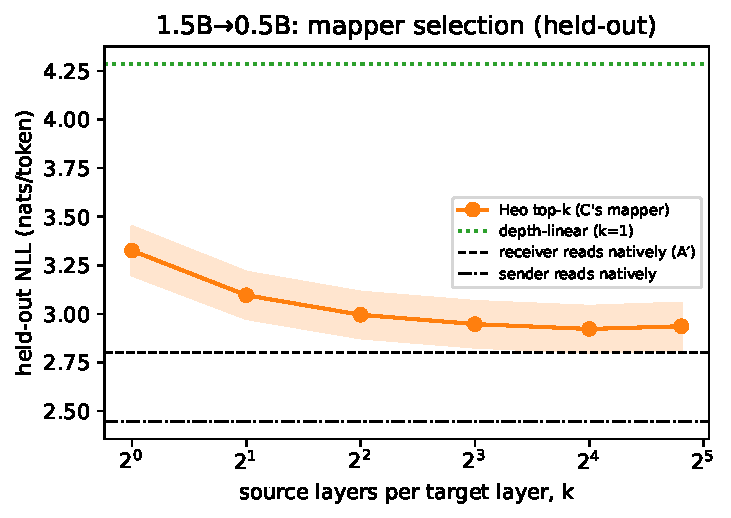
\includegraphics[width=\linewidth]{../figures/paper/fit_ksweep.pdf}
\caption{Held-out prefix-KV NLL against the number of source layers $k$ used by the closed-form mapper of~\citep{heo2026crossmodel}, with 95\% CIs.
Dashed: the receiver reading the same prefix natively (what re-prefill achieves). Dash-dot: the sender reading it natively.}
\label{fig:ksweep}
\end{figure}

\subsection{Transfer cost against switch position}\label{sec:results-intrinsic}
\pending{measurements for this subsection.}


\begin{figure}[t]\centering
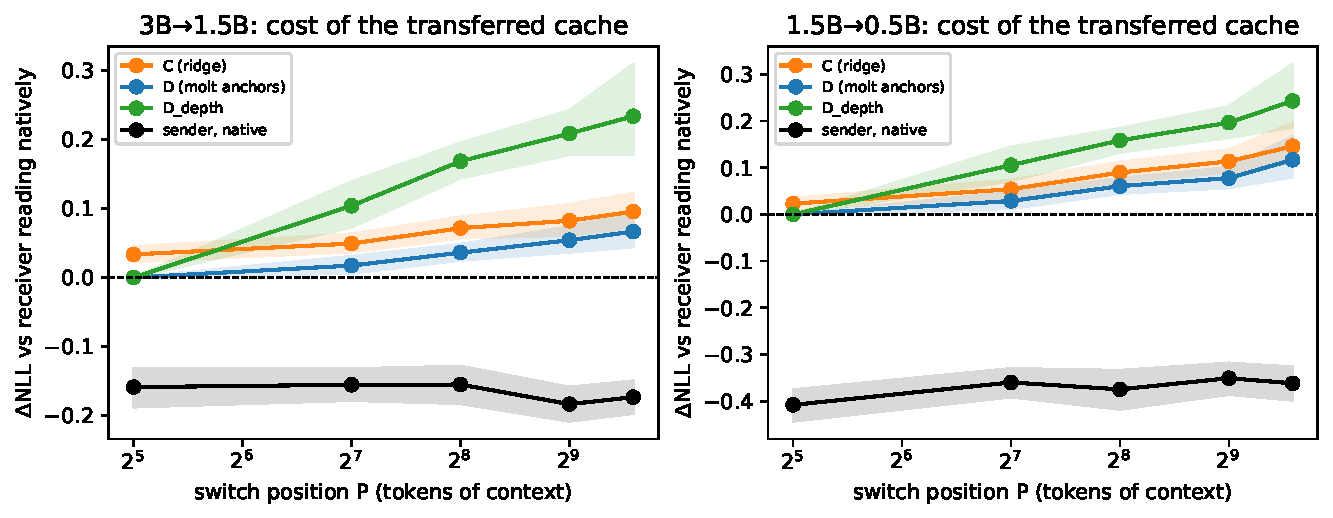
\includegraphics[width=\linewidth]{../figures/paper/intrinsic_context.pdf}
\caption{Experiment I. Extra NLL of the receiver decoding from a transferred cache, relative to reading the same text natively, as a function of how much context precedes the switch. Bands are paired 95\% CIs over evaluation documents.}
\label{fig:intrinsic}
\end{figure}

\subsection{Quality when the switch lands mid-decode}\label{sec:results-quality}
\pending{measurements for this subsection.}


\begin{figure}[t]\centering

\includegraphics[width=\linewidth]{../figures/paper/quality.pdf}
\caption{Experiment Q. GSM8K and needle exact match, and judge top-1 agreement after the switch, per condition. Error bars are 95\% bootstrap CIs.}
\label{fig:quality}
\end{figure}

\subsection{Survival under a per-process limit}\label{sec:results-memory}
\pending{measurements for this subsection.}


\begin{figure}[t]\centering
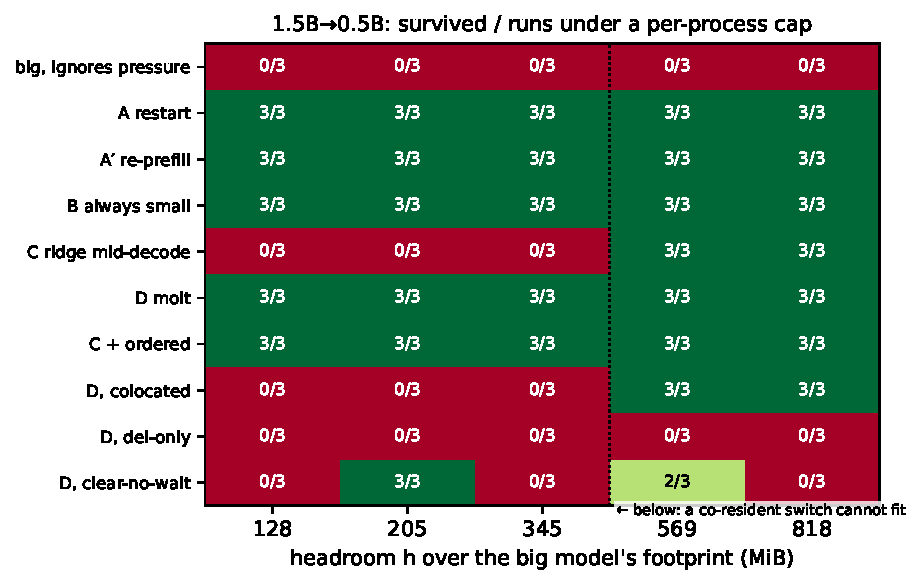
\includegraphics[width=\linewidth]{../figures/paper/memory_survival.pdf}
\caption{Experiment M. Survival rate against headroom $h$ over the big model's own footprint, one process per run under the jetsam emulator. The dotted line marks the headroom a co-resident switch needs (receiver weights $+$ mapper $+$ margin).}
\label{fig:survival}
\end{figure}

\begin{table}[t]\centering\small
\caption{Memory schedules. All of them compute the same transfer; they differ only in what is resident when.}
\label{tab:schedules}
\begin{tabular}{lll}\toprule
schedule & order & resident at peak \\\midrule
colocated & load receiver, map, drop sender & sender $+$ receiver $+$ mapper \\
del-only & drop sender refs, map, load receiver & sender (cached by MLX) $+$ receiver \\
clear-no-wait & drop, \texttt{clear\_cache()}, load at once & depends on reclaim timing \\
ordered & drop, sync, clear, \emph{wait}, map, drop mapper, load & $\max(\text{sender}, \text{KV}+\text{mapper}, \text{receiver})$ \\
\bottomrule\end{tabular}
\end{table}
